\documentclass{article}
% Packages
\usepackage{graphicx,subfig,float} % Required for inserting images
\usepackage{changepage}
\usepackage{amsmath}
\usepackage{datetime}
\usepackage[spanish]{babel}
\usepackage{titling}
\usepackage{geometry}

\geometry{
  a4paper,
  total={170mm,257mm},
  width=150mm,
  height=230mm,
}

\usepackage{tcolorbox}

\graphicspath{{assets/}}

\numberwithin{equation}{section}
\renewcommand{\theequation}{\arabic{section}.\arabic{equation}}

\newenvironment{subs}
  {\adjustwidth{3em}{0pt}}
  {\endadjustwidth}

\providecommand{\abs}[1]{\lvert#1\rvert}


\title{Apuntes \\ Conceptos de Arquitectura de Computadoras}
\author{}
\date{30 de febrero de 2052}

\begin{document}

\maketitle

\newpage
\tableofcontents
\newpage

\section{Introducción a la Arquitectura de Computadoras}

Cuando se describe un computador, frecuentemente se distingue entre \textit{arquitectura} y \textit{organización}.

La \textit{arquitectura} de computadoras se refiere a los atributos de un sistema que son visibles a un programador, o para decirlo de otra manera,aquellos atributos que tiene un impacto directo en la ejecución lógica de un programa.
En cambio, la \textit{organización} de computadores se refiere a las unidades funcionales y sus interconexiones, que dan lugar a especificaciones arquitectónicas.

\subsection{Arquitectura Von Neumann}

La tarea de cargar y modificar programas para el ENIAC\footnote{Electronic Numerical Integrator And Computer, diseñado y contruido bajo la supervisión de John Mauchly y John Presper Eckert en la Universidad de Pennsylvania, fue el primer computador electrónico de propósito general del mundo.} era extremadamente tediosa. El proceso de programación podría ser más fácil si el programa se representara en una forma adecuada parta ser guardado en la memoria junto con los datos.
Esta idea conocida como \textit{concepto de programa-almacenado}, se atribuye al matemático y físico alemán John von Neumann.

La \textbf{unidad central de procesamiento (CPU)} está constitutida por la \textbf{unidad de control (UC)} y la unidad \textbf{aritmético-lógica (ALU)}.
Los datos e instrucciones deben introducirse en el sistema y los resultados se proporcionarán mediante componentes de \textbf{entrada/salida (E/S)}.
Para almacenar temporalmente los datos e instrucciones, se utiliza una \textbf{memoria principal}.

\begin{figure}[h]
  \centering
  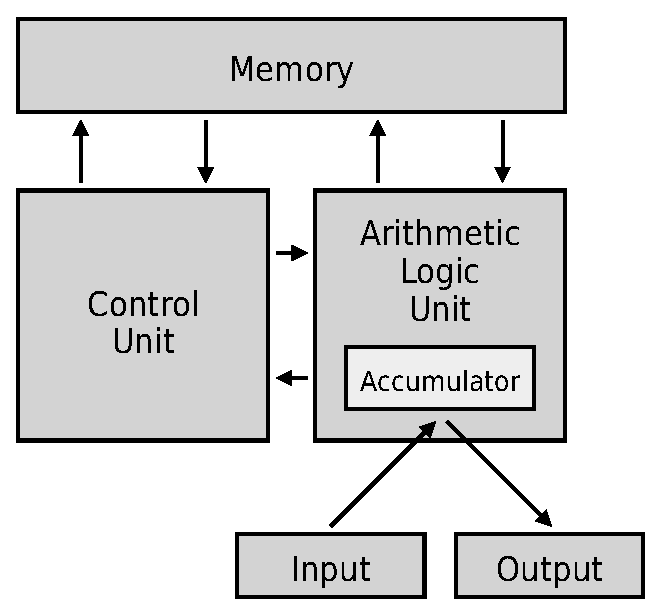
\includegraphics[width=0.6\textwidth]{Von_Neumann_architecture}
  \caption{Arquitectura Von Neumann}
\end{figure}
\subsection{Repertorio de instrucciones}

El funcionamiento del procesador está determinado por las instrucciones que ejecuta. Estas instrucciones se denominan \textit{instrucciones de maquina}. Al conjunto de instrucciones distintas quepuede ejecutar el procesador se denomina \textit{repertorio de instrucciones}.

\begin{subs}
  \subsubsection{Elementos de las instrucciones de maquina}

  Cada instrucción debe contener la información que necesita el procesador para su ejecución. Dichos elementos son:

  \begin{itemize}
    \item \textbf{Código de operación}: especifica la operación a realizar (suma, E/S, etc.).
    \item \textbf{Referencia a operandos fuente u origen}: la operación puede implicar a uno o más operandos origen, es decir operandos que son entradas para la instrucción.
    \item \textbf{Referencia al operando de destino}: la operación puede producir un resultado que debe ser almacenado en un operando destino.
    \item \textbf{Referencia a la siguiente instrucción}: especifica la ubicación de la siguiente instrucción a ejecutar, (generamente la misma está implicita).
  \end{itemize}

  La siguiente instrucción a captar está en memoria principal o, en el caso de un sistema de memoria virtual, bien en memoria principal.
  Los operandos origen y destino pueden estar en alguna de las tres áreas siguientes:

  \begin{itemize}
    \item \textbf{Memoria principal o virtual}: como en las referencias a instrucciones siguientes, debe indicarse la dirección de memoria principal.
    \item \textbf{Registro del procesador}: un procesador contiene uno o más registros que pueden ser referenciados por instrucciones máquina.
    \item \textbf{Dispositivo de E/S}: la instrucción debe especificar el módulo y dispositivo de E/S para la operación.
  \end{itemize}

  \begin{figure}[H]
    \centering
    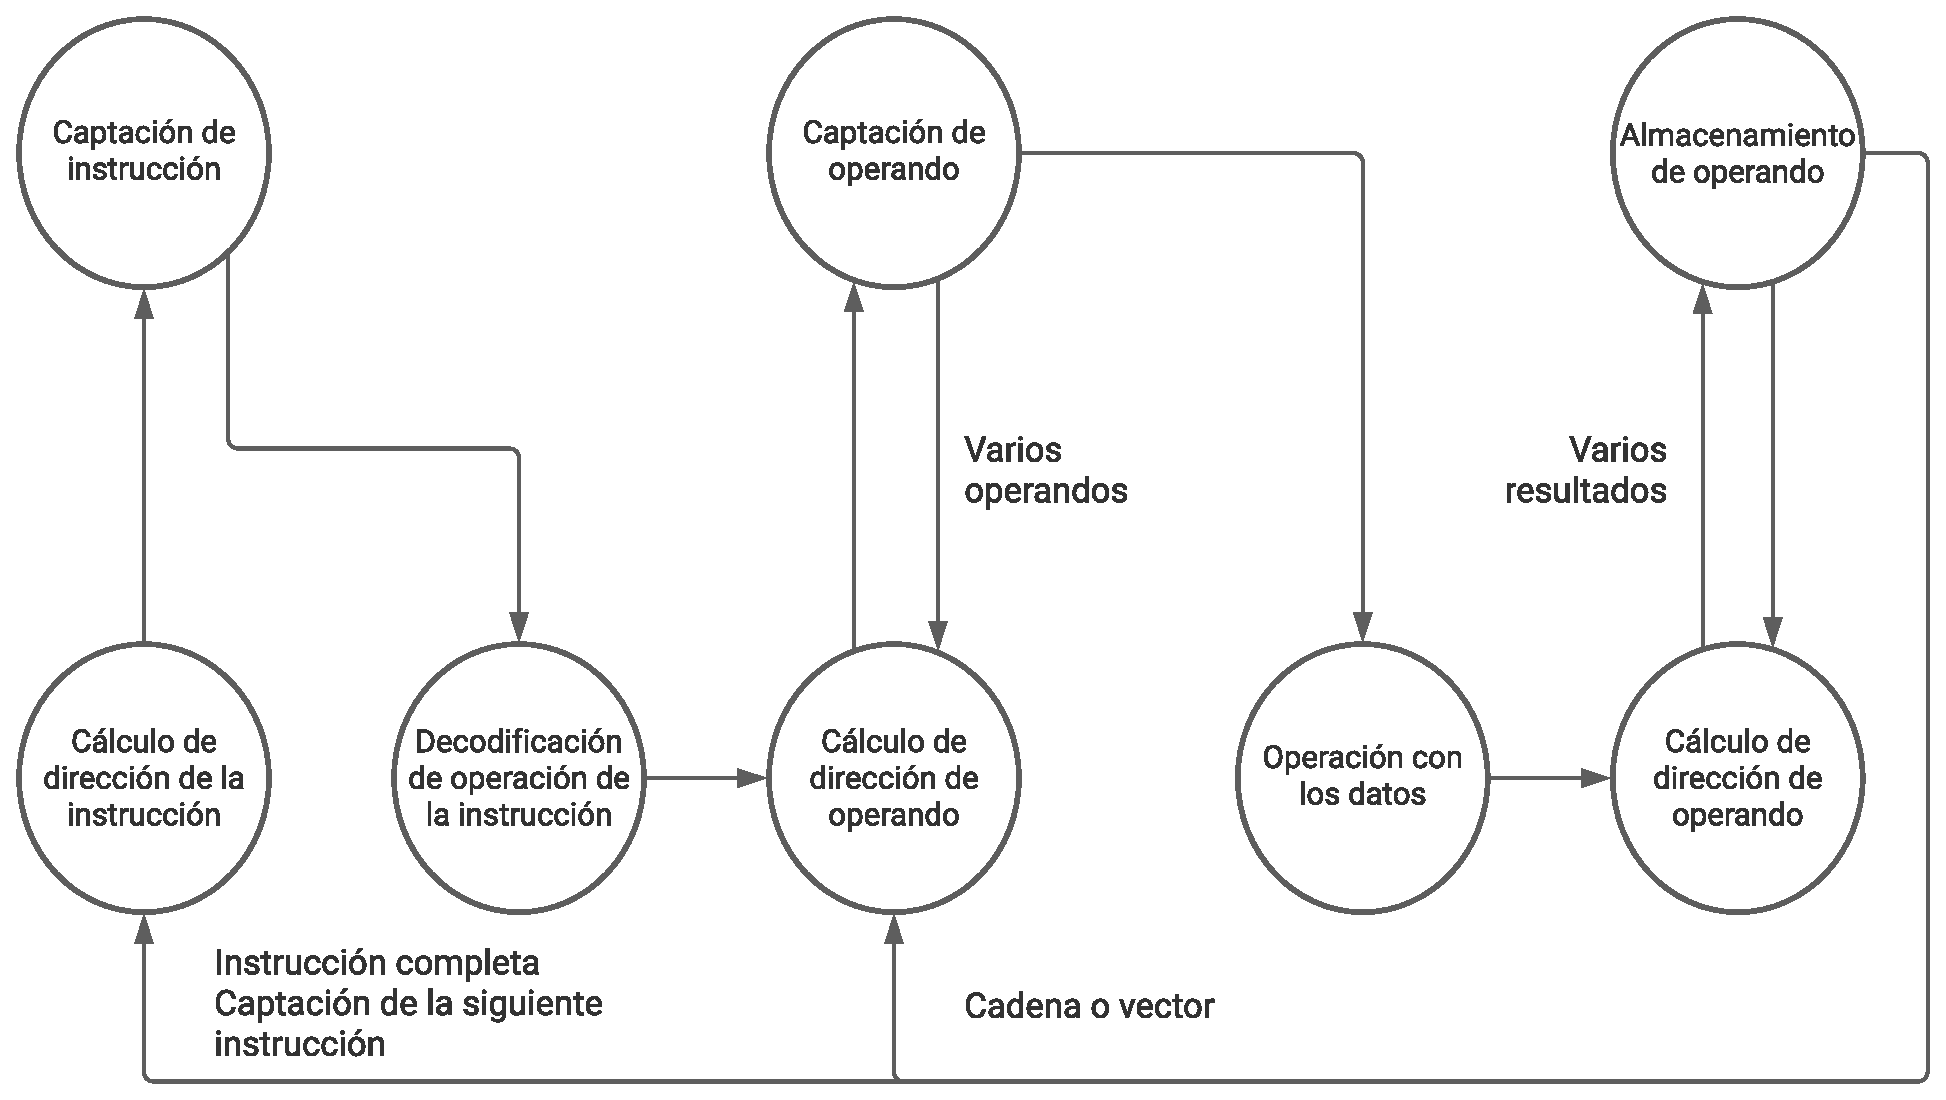
\includegraphics[width=0.8\textwidth]{Ciclo-de-instruccion-CLI}
    \caption{Ciclo de instrucción}
  \end{figure}

  \subsubsection{Tipos de instrucciones}

  Cualquier programa escrito en alto nivel debe traducirse a lenguaje máquina para ser ejecutado. El repertorio de instrucciones máquina debe ser suficientemente amplio como para expresar cualquiera de las instrucciones e un lenguaje de alto nivel. Teniendo esto presente, los tipos de instrucciones se pueden clasificar de la siguiente manera:
  \begin{itemize}
    \item \textbf{Procesamiento de datos}: son instrucciones aritméticas y lógicas.
    \item \textbf{Almacenamiento de datos}: son instrucciones de memoria.
    \item \textbf{Transferencia de datos}: son instrucciones de E/S.
    \item \textbf{Control}: son instrucciones de comprobación y bifurcación.
  \end{itemize}

  Las instrucciones \textit{aritméticas} proporcionan capacidad computacional para procesar datos numéricos. Las instrucciones \textit{lógicas} operan con los bits de una palabra en lugar considerarlos como números. Las instrucciones \textit{memoria} permiten transferir los datos entre la memoria y los registros. Las instrucciones \textit{E/S} se necesitan para transferir programas y datos a memoria y devolver resultados de los cálculos al usuario.

  \subsubsection{Número de direcciones}

  Una de las formas tradicionales de describir la arquitectura de un procesador es en términos del número de direcciones contenidas en cada instrucción. Esta dimensión se va haciendo menos significativa a medida que aumenta la complejidad del diseño del procesador.

  La mayoria de las instrucciones tienen una, dos o tre direcciones, estando implicita la dirección de la instrucción siguiente (obtenida a través del contador de programa)

  \begin{itemize}
    \item \textbf{Instrucciones de una dirección}: para funcionar, una segunda dirección debe estar implícita. La dirección implícita es el registro del procesador \textit{acumulador}. El acumulador contiene uno de los operandos y se emplea para almacenar el resultado.
    \item \textbf{Instrucciones de dos direcciones}: para operaciones binarias una de las direcciones debe hacer el servicio doble de uno de los operandos y del resultado.
    \item \textbf{Instrucciones de tres direcciones}: no son comunes ta que requieren formatos relativamente largos para albergar las tres referencias. Una dirección es el destino y las otras dos son los operandos.
  \end{itemize}

  \subsubsection{Diseño del repertorio de instrucciones}

  El repertorio de instrucciones es el medio que tiene el programador para controlar el procesador. En consecuencia deben considerarse las necesidades del programador a la hora de diseñar el repertorio de instrucciones.

  Los aspectos fundamentales de diseño más importantes son:

  \begin{itemize}
    \item El \textbf{repertorio de operaciones}: cuántas y qué operaciones considerar, cuán complejas deben ser.
    \item Los \textbf{tipos de datos}: los distintos tipos de datos con los que se efectúan operaciones.
    \item Los \textbf{formatos de instrucciones}: longitud de la instrucción (en bits), número de direcciones, tamaño de los distintos campos, etc.
    \item Los \textbf{registros}: número de registros del procesador que pueden ser referenciados por las instrucciones, y su uso.
    \item El \textbf{direccionamiento}: el modo o modos de direccionamiento mediante los cuales puede especificarse la dirección de un operando.
  \end{itemize}

\end{subs}

\subsection{Tipos de operando}

Las instrucciones máquina operan con datos. Las categorías más importantes de datos son:

\begin{itemize}
  \item Direcciones
  \item Números 
  \item Caracteres
  \item Datos lógicos
\end{itemize}

\begin{subs}
  \subsubsection{Direcciones}

  \subsubsection{Números}

  En los computadores son usuales tres tipos de datos numéricos:

  \begin{itemize}
    \item Enteros o en coma fija.
    \item En coma flotante.
    \item En decimal.
  \end{itemize}

  Hay que aclarar que hay un límite para la magnitud de los números representables en una máquina y en el caso de números de coma flotante, su precisión está limitada. Por tanto, el programador debe ser consciente de las consecuencias del redondeo, el desbordamiento o el desbordamiento a cero.

  \subsubsection{Caracteres}

  Una forma bastante común de datos es el texto o secuencieas de caracteres. Aunque la información textual sea más conveniente para las personas, los computadores trabajan mejor con números. Por tanto, los caracteres se representan mediante números. En la mayoría de los sistemas, los caracteres se representan mediante un código de 8 bits. El código ASCII\footnote{American Standard Code for Information Interchange} es el más común.

  \subsubsection{Datos lógicos}

  A veces resulta útil considerar una unidad de \textit{n} bits como \textit{n} elementos o datos de un bit, donde cada elemento tiene un valor de 1 o 0. Cuando los datos son vistos de esta manera, se consideran datos \textit{lógicos}.
  Las principal ventaja es que nos permiten almacenar una matriz de elementos bianarios o booleanos, por lo que la memoria puede ser utilizada de forma eficiente. También hay ocasiones en las que queremos manipular bits individuales de un dato.
\end{subs}

\subsection{Orden de los bytes}

Supongamos una memoria direccionable de a byte, es decir, que cada byte tiene un dirección única. ¿Cómo se leeran los números que ocupan más de un byte? ¿Cómo se escribirán los números que ocupan más de un byte? 
Para este problema se crearon dos formatos de almacenamiento:

\begin{itemize}
  \item \textbf{Big endian}: el byte más significativo se almacena en la dirección con valor numérico más bajo.
  \item \textbf{Little endian}: el byte menos significativo se almacena en la dirección con valor numérico más bajo.
\end{itemize}

\begin{figure}[H]
  \hspace*{\fill}
  \subfloat[Big endian]{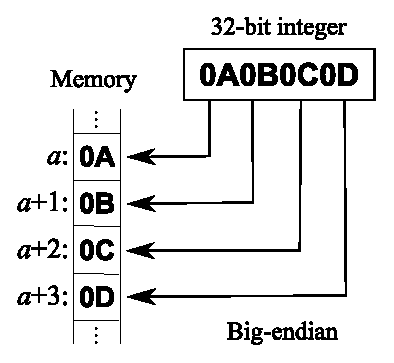
\includegraphics[width=0.30\textwidth]{Big-Endian}}
  \hfill
  \subfloat[Little endian]{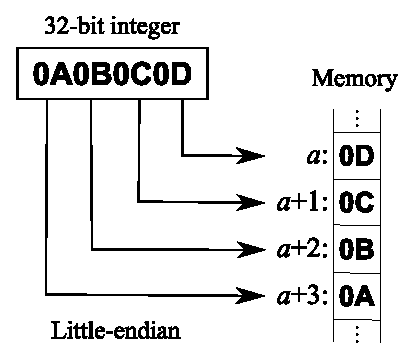
\includegraphics[width=0.30\textwidth]{Little-Endian}}
  \hspace*{\fill}
\end{figure}

\subsection{Modos de direccionamiento}

El campo o campos de direcciones en un formato de instrucción usual está bastante limitado. Para poder referenciar un rango elevado de posiciones se han empleado diversas técnicas de direccionamiento. Las más comunes son:

\begin{itemize}
  \item \textbf{Inmediato}
  \item \textbf{Directo}
  \item \textbf{Indirecto}
  \item \textbf{Registro}
  \item \textbf{Indirecto con registro}
  \item \textbf{Indirecto con desplazamiento}
  \item \textbf{Pila}
\end{itemize}

\begin{subs}
  \subsubsection{Inmediato}
  El operando se encuentra presente en la propia instrucción. La ventaja es que una vez captada la instrucción, no se requiere una referencia a memoria para obtener un operando. La desventaja es que el tamaño del número está restringido a la longitud del campo de direcciones.

  \subsubsection{Directo}

  El campo de direcciones contiene la dirección efectiva del operando. La ventaja es que solo se requiere una referencia a memoria y no necesita ningún cálculo especial. La limitación es que proporciona un espacio de direcciones restringido.

  \subsubsection{Indirecto}

  El campo de direcciones referencia a la dirección de una palabra en memoria, la cual contiene la dirección completa del operando.

  La ventaja de esta aproximación es que para una longitud de palabra $N$bits, se dispone ahora un espacio de direcciones de $2^N$. La desventaja es que la ejecución de la instrucción requiere dos referencias a memoria para captar el operando.

  \subsubsection{Registro}

  El campo de direcciones contiene el número de registro que contiene el operando. La ventaja es que la ejecución de la instrucción no requiere ninguna referencia a memoria. La desventaja es que el número de registros es limitado.

  \subsubsection{Indirecto con registro}

  El campo de direcciones contiene el número de registro que contiene la dirección del operando. La ventaja es que la ejecución de la instrucción requiere una referencia a memoria. La desventaja es que el número de registros es limitado.

  \subsubsection{Indirecto con desplazamiento}

  El direccionamiento con desplazamiento requiere que las instrucciones tengan dos campos de direcciones, al menos uno de los cuales explícito. El valor contenido en uno de los campos de direcciones se utiliza directamente. El otro campo, se refiere a un registro cuyo contenido se suma al valor del campo de direcciones. El resultado de la suma se utiliza como la dirección del operando.

  \begin{itemize}
    \item \textbf{Direccionamiento relativo}: el registro referenciado implícitamente es el \textbf{PC}. 
    \item \textbf{Direccionamiento con registro base}: el registro referenciado contiene una dirección de memoria, y el campo de dirección contiene un desplazamiento desde dicha dirección. La referencia a registro puede ser explícita o implícita.
    \item \textbf{Indexado}: el campo de dirección referencia una dirección de memoria principal, y el registro referenciado contiene un desplazamiento positivo desde esa dirección.
  \end{itemize}

  \subsubsection{Pila}

  El modo de direccionamiento de pila, (explicado en el Apéndice\ref{ap:pilas}), es una forma de direccionamiento implícito. Las instrucciones máquina no necesitan incluir una referencia a memoria sino que operan implícitamente con la cabecera de la pila.
\end{subs}

\subsection{Tipos de operaciones}

Las operaciones que se pueden realizar en un computador se pueden clasificar en:

\begin{itemize}
  \item \textbf{Transeferencia de datos}: mueven datos entre registros, registros a memoria y memoria a registros. Se debe especificar la ubicacion del operando fuente y destino, el tamaño de los datos y el modo de direccionamiento.
  \item \textbf{Aritméticas}: son las operaciones ADD, SUB, MUL y DIV.\@ Puede incluirse tambien las operaciones INC o DEC (que solamente necesitan un operando), NEG (cambia el signo en Ca2) y ABS (valor absoluto).
  \item \textbf{Lógicas}: son las operaciones AND, OR, XOR, NOT.\@ Puede incluirse tambien las operaciones SHL, SHR, ROL, ROR (que solamente necesitan un operando).
  \item \textbf{Conversión}: son operaciones para cambiar formatos de datos, por ejemplo de EBCDIC\footnote{Extended Binary Coded Decimal Interchange Code} a ASCII.\@
  \item \textbf{E/S}: son operaciones para leer o escribir datos en dispositivos de E/S. Son las instrucciones IN y OUT.\@ Se pueden realizar a través de un controlador aparte \textit{DMA}\footnote{Direct Memory Access}.
  \item \textbf{Control}: son las instrucciones de salto, llamadas a subrutinas, etc. Algunas de ellas pueden ser JMP, JZ, JNZ, CALL, RET, etc.
\end{itemize}

\subsection{Organización del procesador}

Para comprender la organización del procesador, consideremos los requisitos que ha de cumplir:

\begin{itemize}
  \item \textbf{Captar instrucción}: el procesador lee una instrucción de la memoria.
  \item \textbf{Interpretar instrucción}: la instrucción se decodifica para determinar qué acción es necesaria.
  \item \textbf{Captar datos}: la ejecución de una instrucción puede exigir leer datos de la memoria o de un módulo de E/S.
  \item \textbf{Procesar datos}: la ejecución de una instrucción puede exigir llevar a cabo alguna operación aritmética o lógica.
  \item \textbf{Escrbibir datos}: los resultados de una ejecución pueden exigir escribir datos en la memoria o en un módulo de E/S.
\end{itemize}

\subsection{Organización de los registros}

Los registros del procesador son de dos tipos:

\begin{itemize}
  \item \textbf{Registros visibles por el usuario}: permiten a programador de lenguaje máquina minimizar las referencias a memoria principal por medio de la optimización del usa de registros.
  \item \textbf{Registros de control y de estado}: son utilizador por la unidad de control para controlar el funcionamiento del procesador y por programas privilegiados del sistema operativo para controlar la ejecución de programas.
\end{itemize}

\begin{subs}
  \subsubsection{Registros visibles por el usuario}
  Un registro visible por el usuario es aquél que puede ser referenciado por medio del lenguaje máquina que ejecuta el procesador.

  Los \textbf{registros de uso general} pueden ser asignados por el programador a diversas funciones. Su uso dentro del repertorio de instrucciones puede ser ortogonal a la operación. Por ejemplo, el registro $R_0$ puede ser usado como un registro de acumulación, un registro de índice o un registro de apuntador.

  Los \textbf{registros de datos} pueden usarse unicamente para contener datos y no se pueden emplear en el cálñculo de la dirección de un operando.

  Los \textbf{registros de dirección} pueden ser de uso más o menos general, o pueden estar dedicados a un modo de direccionamiento particular.

  Los \textbf{registros de código de condición} son bits fijados por el hardware del procesador como resultado de alguna operación. Estos bits son usados por el programador para controlar el flujo de ejecución de un programa.

  \subsubsection{Registros de control y de estado}

  Hay diversos registros del procesador que se emplean para controlar su funcionamiento. La mayoría de ellos, no son visibles por el usuario. 
  Para la ejecución de una instrucción son esenciales cuatro registros:

  \begin{itemize}
    \item \textbf{PC}: contiene la dirección de la instrucción que se está ejecutando.
    \item \textbf{IR}: contiene la instrucción que se está ejecutando.
    \item \textbf{MAR}: contiene la dirección de memoria que se está accediendo.
    \item \textbf{MBR}: contiene la palabra de datos a escribir en memoria o la palabra leída más recientemente.
  \end{itemize}
\end{subs}

\subsection{Ciclo de instrucción}

El ciclo de instrucción es el conjunto de operaciones que se llevan a cabo para ejecutar una instrucción. El ciclo de instrucción se divide en tres etapas:

\begin{itemize}
  \item \textbf{Captación}: llevar la siguiente instrucción de la memoria al procesador.
  \item \textbf{Ejecución}: interpretar el código de operación y llevar a cabo la operación indicada.
  \item \textbf{Interrupción}: si las interrupciones están habilitadas y ha ocurrido una interrupción, guardar el estado del proceso actual y atender la instrucción.
\end{itemize}
\section{Interrupciones}

Con el uso de interrupciones, el procesador puede dedicarse a ejecutar otras instrucciones mientras una operación de E/S está en curso. El procesador puede ser notificado cuando la operación de E/S ha terminado, y puede continuar con la ejecución de la instrucción que se interrumpió.
Cuando el dispositivo externo está listo para aceptar maás datos del procesador, el módulo de E/S de este dispositivo externo envía una señal de \textit{petición de interrupción} al procesador. El procesador responde suspendiendo la operación del programa que estaba ejecutando y salta a un programa, conocido como gestor de interrupción, que da servicio a ese dispositivo concreto, y prosigue con la ejecución del programa original después de haber dado dicho servicio al dispositivo.

Para permitir el uso de interrupciones, se añade un \textit{ciclo de interrupción} al ciclo de instrucción. En el ciclo de interrupción el procesador comprueba si se ha generado alguna interrupción, indicada por la presencia una señal de interrupción. Si no hay señales, el procesador contonúa con el ciclo de captación y accede a la siguiente instrucción del programa. Si hay alguna petición, el procesador suspende la ejecución del programa en curso y guarda su contexto. El procesador carga el contador de programa con la dirección de comiento de una rutina de interrupción.

\begin{figure}[h]
  \centering
  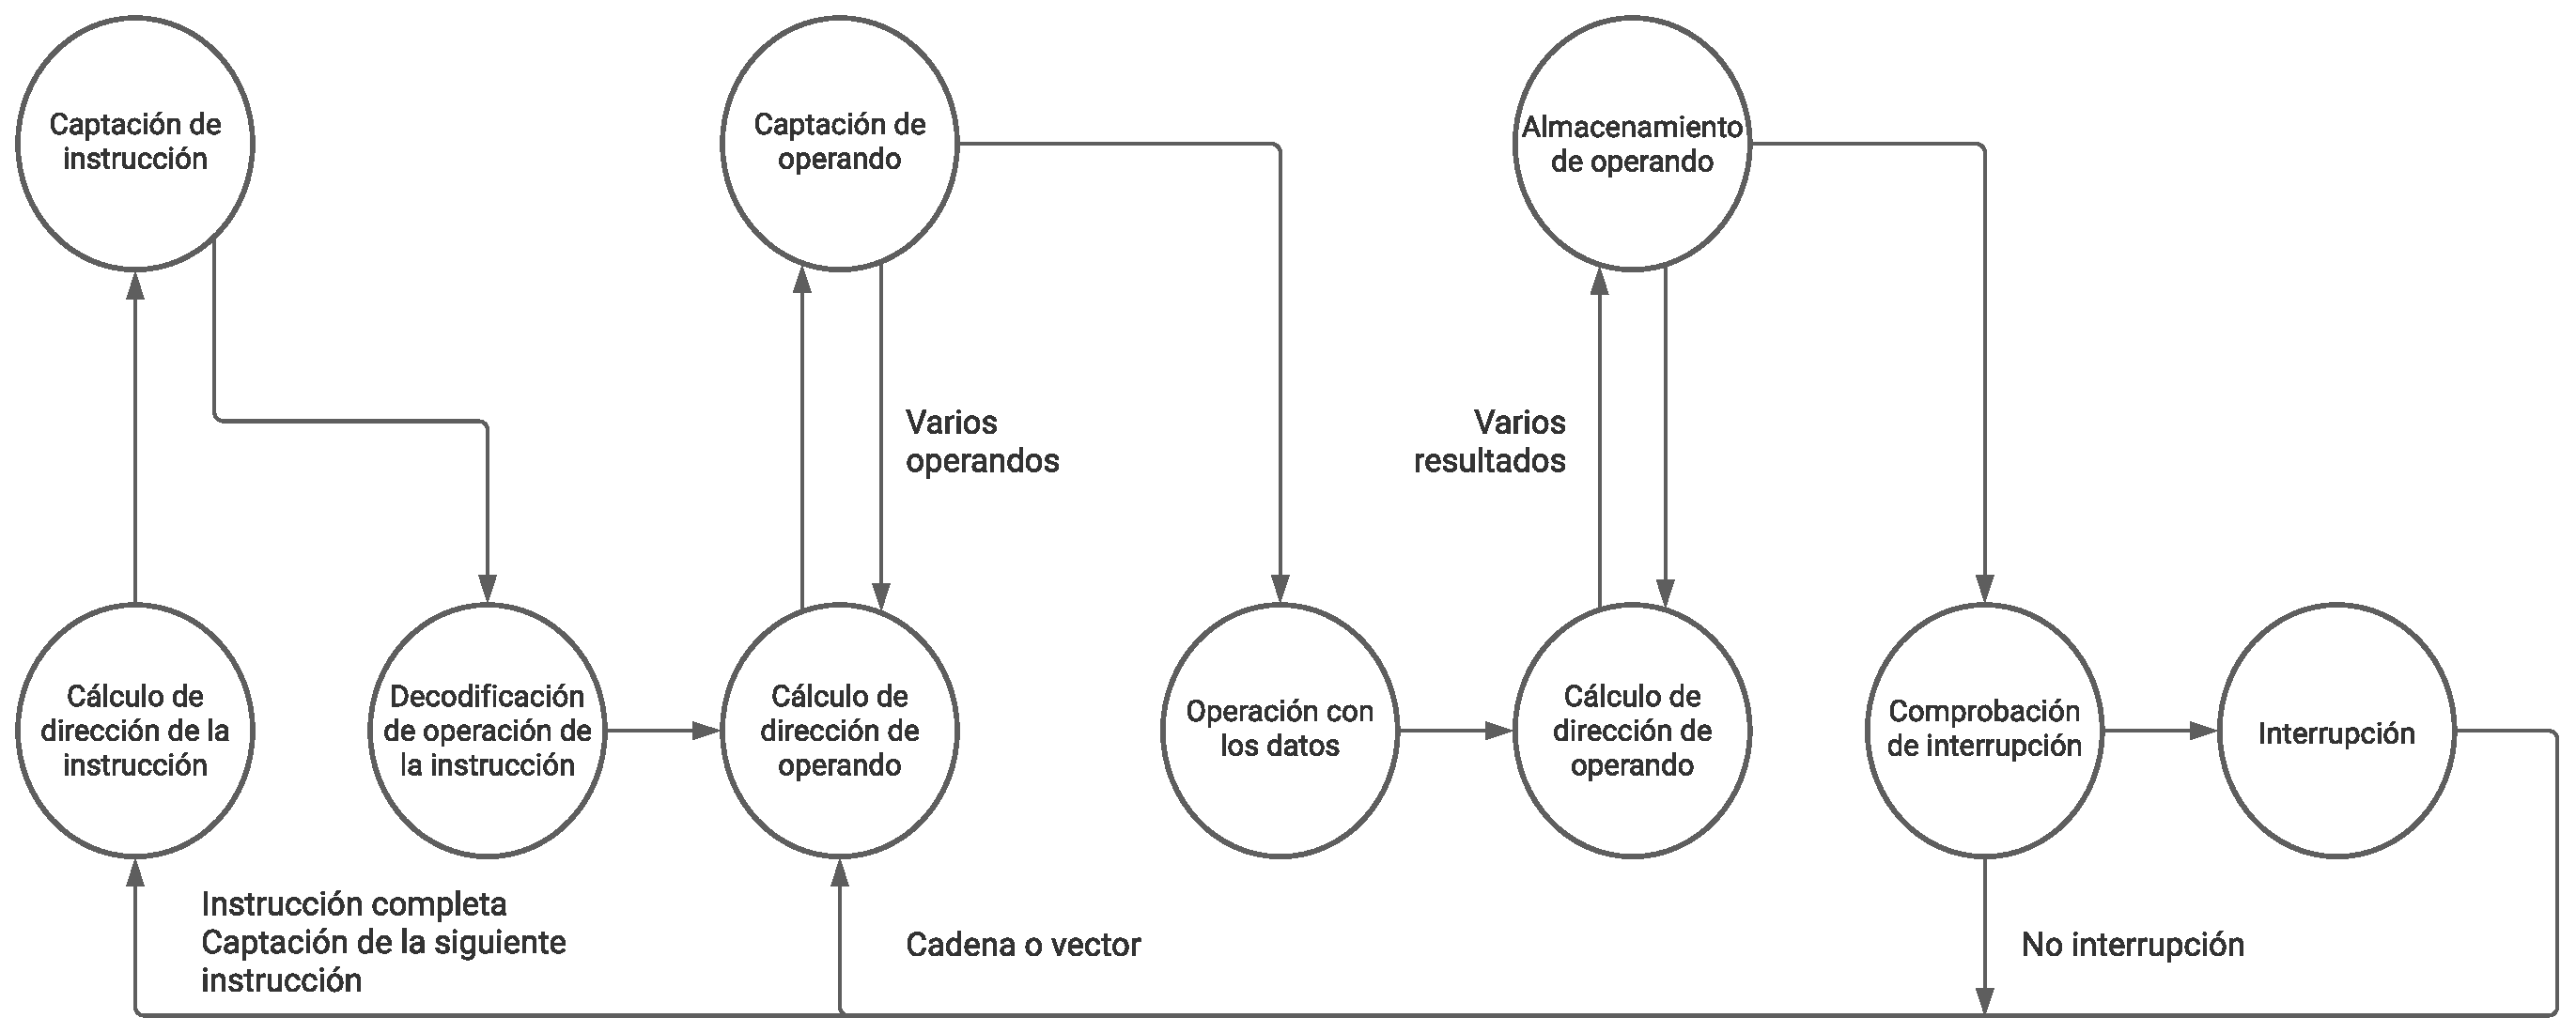
\includegraphics[width=0.8\textwidth]{Ciclo-de-instruccion-STI}
  \caption{Ciclo de instrucción (con interrupciones)}
\end{figure}

\subsection{Tipos de interrupciones}

Podemos clasificar las interrupciones dependiendo de su importancia:

\begin{itemize}
  \item \textbf{No enmascarables}: son aquellas interrupciones que no pueden ser ignoradas. Indican eventos peligros o de alta prioridad y requieren un respuesta eficiente y rápida.
  \item \textbf{Enmascarables}: son aquellas interrupciones que pueden ser ignoradas. Sus eventos no configuran peligro ó pueden esperar. La posible solicitud de interrución puede inhibirse con instrucciones especiales.
\end{itemize}

\begin{subs}
  \subsubsection{Interrupciones por hardware}
  
  Las interrupciones por hardware son las generadas por los dispositivos de E/S. El sistema de cómputo tiene que manejar estos eventos externos `no planeados`. Además, las mismas no están relacionadas con el proceso que se encuentra ejecutándose en ese momento. Son conocidas como \textit{interrupt request}.

  Las \textbf{traps/excepciones} son interrupciones por hardware creadas por el procesador moderno en respuesta a ciertos eventos internos:

  \begin{itemize}
    \item \textbf{Condiciones excepcionales}: overflow en el ALU de punto flotante.
    \item \textbf{Falla de programa}: tratar de ejecutar una instrucción no definida.
    \item \textbf{Falla de hardware}: error de paridad de memoria.
    \item \textbf{Accesos no alineados ó a zonas de memoria protegidas}: acceso a memoria no permitido.
  \end{itemize}

  \subsection{Interrupciones por software}

  Las interrupciones por software son instrucciones explícitas que afectan al procesador de la misma manera que las interrupciones por hardware. La instrucción INT $n$ permite a las interrupciones ser generadas desde dentro del software utilizando el número del vector de interrupción como un operando.

  Estas interrupciones permiten depurar los gestores de interrupción. También se utilizan para invocar funciones del sistema operativo, permitiendo asi cargar subrutinas del sistema operativo en algún lugar y puedan utilizarse.
\end{subs}

\subsection{Interrupciones múltiples}

Hasta ahora únicamente se ha discutido la existencia de una sola interrupción. Sin embargo, es posible que se produzcan varias interrupciones simultáneamente. 
Se pueden seguir dos alternativas para tratar las interrupciones múltiples:

\begin{itemize}
  \item \textbf{Interrupción inhabilitada}: mientras se está atendiendo una interrupción, se deshabilitan las interrupciones. Si se produce una interrupción, queda pendiente y será examinada por el procesador una vez que este haya activado las interrupciones nuevamente.
  El inconveniente de este enfoque es que no teiene en cuenta la prioridad relativa ni las solicitudes con un tiempo crítico. 
  \item \textbf{Interrupciones con prioridades}: se defienen prioridades para las interrupciones y permite que una interrupción de prioridad más alta pueda interrumpir a un gestor de interrupción de prioridad menor. Cuando se ha gestinoado la interrupción de prioridad más alta, el procesador vuelve a las interrupciones previas.
\end{itemize}

\begin{figure}[H]
  \centering
  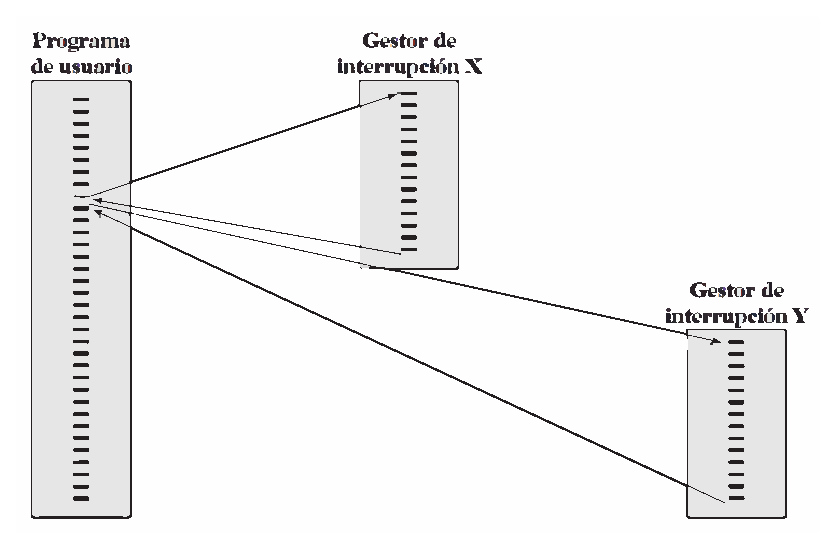
\includegraphics[width=0.8\textwidth]{Interrupciones-secuenciales}
  \caption{Interrupciones secuenciales}
\end{figure}

\begin{figure}[H]
  \centering
  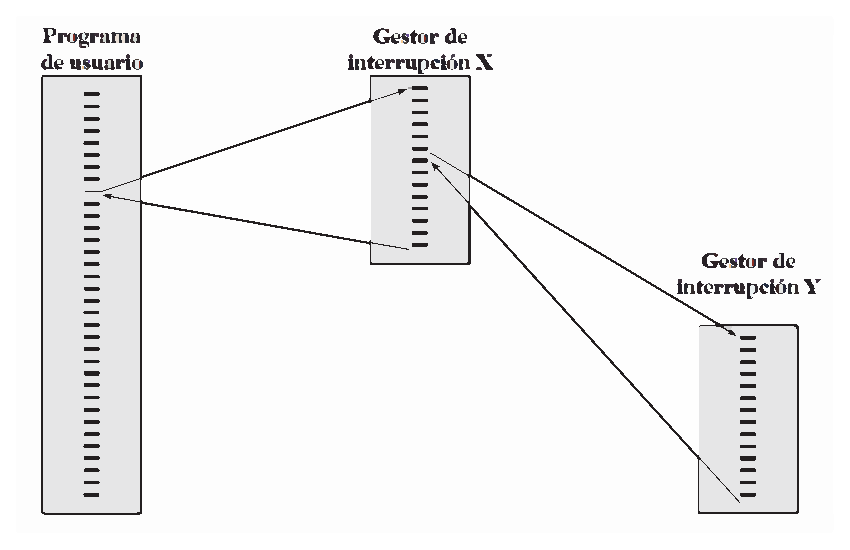
\includegraphics[width=0.8\textwidth]{Interrupciones-anidadas}
  \caption{Interrupciones con prioridades}
\end{figure}

\subsection{Funcionamiento de las E/S}

Un módulo de E/S puede intercambiar datos directamente con el procesador. Igual que el procesador puede iniciar una lectura o escritura en memoria, también puede leer o escribir datos de un módulo de E/S.
En algunos casos, es deseable permitir que los intervambios de E/S se produzcan directamente con la memoria. En ese caso, el procesador cede a un módulo de E/S la autoriadad para leer de o escribir en memoria, para que así la transferencia de E/S-memoria pueda producirse sin la intervención  sel procesador.
Durante esas transferencias, el módulo de E/S proporciona a la memoria las órdenes de lectura o escritura, liberando al procesador de cualquier responsabilidad en el intercambio. Esta operación se conoce con el nombre de \textit{DMA} (Direct Memory Access).

\subsection{Reconocimiento de interrupciones}

\begin{itemize}
  \item \textbf{Interrupciones multinivel}: cada dispositivo que puede provocar una interrupción tiene una entrada física de interrupción conectada a la CPU.\@ Es muy sencillo, pero a la vez muy caro.
  \item \textbf{Línea de interrupción única}: hay una sola entrada física de pedido de interrupción a la que están conetados todos los dispositivos. Es necesario preguntar a cada dispositivo si ha producido el pedido de interrupción (técnica de \textit{polling}).
  \item \textbf{Interrupciones vectorizadas}: el dispositivo que quiere interrumpir además de la señal de pedido de interrupción, debe colocar en el bus de datos un identificador.
\end{itemize}

El encargado de manejar todas las interrupciones es el \textbf{PIC}\footnote{Programmable Interrupt Controller}. Las tareas realizas por el PIC son:

\begin{itemize}
  \item Puesto que existen muchos dispositivos que pueden solicitar interrupciones, es responsabilidad del PIC priorizarlas cuando existen varias IRQ's simultáneas.
  \item Después de enviar una solicitud de interrupción, debe enviar un número de interrupción (número de vector) cuando el procesador indica que está listo para atender la petición.
  \item Mantiene un registro de que se está procesando una interrupción; cuando esto no sucede, no envía más peticiones hasta que este le responde con una señal EOI\footnote{End of Interrupt}, indicando que la rutina de servicio precedente ha terminado o puede aceptar otra interrupción.
  \item Puede enmascarar de forma selectiva cualquiera de las 8 IRQ's que tiene conectadas.
\end{itemize}

El \textbf{PIC} tiene varios registros internos, ellos son:

\begin{itemize}
  \item \textbf{EOI}: recibe 20H cuando el procesador ha terminado de atender la interrupción.
  \item \textbf{Interrupt Mask Register}: contiene los bits de máscara de las IRQ's.
  \item \textbf{Interrupt Request Register}: contiene los bits de estado de las IRQ's.
  \item \textbf{Interrupt Status Register}: contiene el bit de estado de la IRQ que se está atendiendo.
  \item \textbf{INT0\ldots INT7}: son los 8 vectores de interrupción.
\end{itemize}
\section{Entrada y salida}

Un módulo de E/S no es únicamente un conector mecánico quie permite encufar el dispositivo al bus del sistema; sino que además está dotado de cierta <<inteligencia>>, que contiene la lógica necesaria para permitir la comunicación entre el periférico y el bus.

Las razones por las que los periféricos no se conectan directamente al bus del sistema son:

\begin{itemize}
  \item Hay una plia variadadd e periféricos con formas de funcionamiento direferentes. Podría ser imposible incorporar la lógica necesaria dentro del procesador para controlar tal diversidad de dispositivos.
  \item Generalmente, la velocidad de transferencia de datos de los periféricos es mucho menor que la de la memoria o el procesador.
  \item Por otro lado, la velocidad de transferencia de algunos periféricos es mayor que la de la memoria o el procesador.
  \item Los periféricos suelen utilizar datos con formatos y tamaños de palabra diferentes de los del computador a los que se conectan.
\end{itemize}

En consecuencia, se necesita un módulo de E/S. Este módulo tiene dos funciones principales:

\begin{itemize}
  \item Realizar la interfaz entre el procesador y la memoria y los periféricos.
  \item Realizar la interfaz entre uno o más dispositivos periféricos.
\end{itemize}

\subsection{Dispositivos externos}

Un dispositivo externo se conecta al computador mediante un enlace a un módulo de E/S. El enlace se utiliza para intercambiar señales de control, estado, y datos entre el módulo de E/S y el dispositivo externo. Los dispositivos externos pueden ser:

\begin{itemize}
  \item \textbf{E/S básicos}: monitor, mouse, teclado, etc.
  \item \textbf{E/S de almacenamiento}: discos duros, CD-ROM, etc.
  \item \textbf{Impresión}: impresoras, escáneres, etc.
  \item \textbf{Comunicaciones}: módems, acceso/interfaz de red, etc.
  \item \textbf{Multimedia}: microfónos, altavoces, etc.
  \item \textbf{Automatización y control}: sensores, alarmas, etc.
\end{itemize}

\begin{figure}[H]
  \centering
  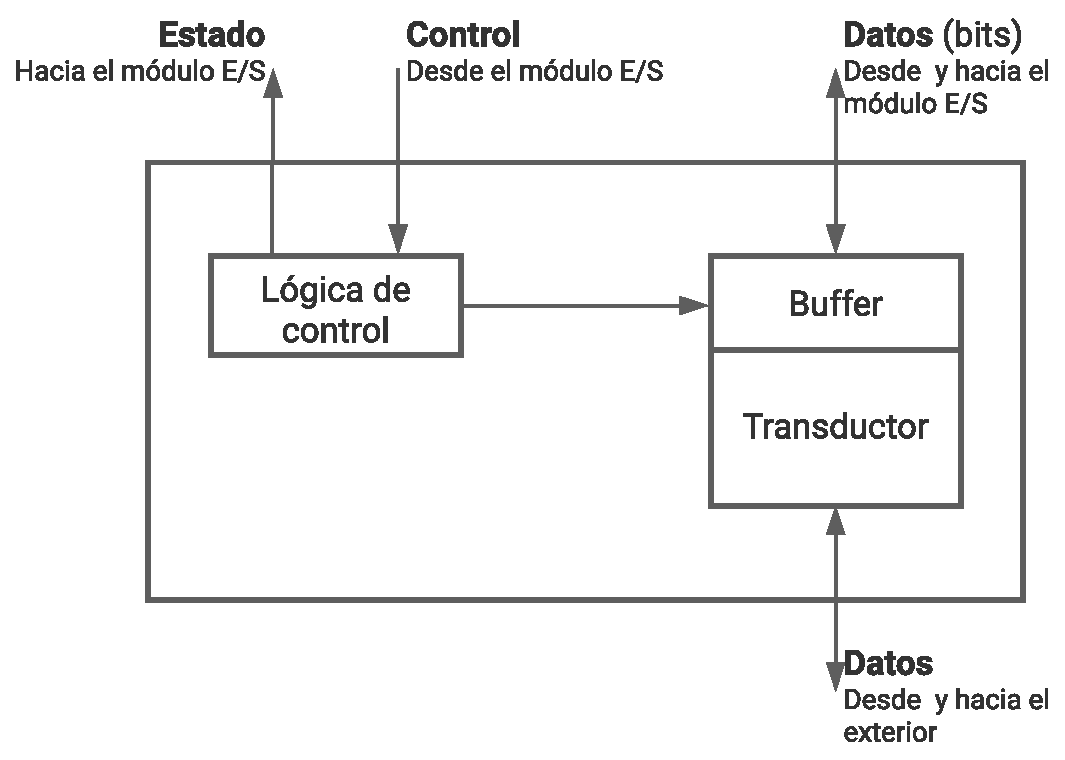
\includegraphics[width=0.6\textwidth]{Dispositivo-externo-tipo}
  \caption{Dispositivo externo}\label{fig:Dispositivo-externo-tipo}
\end{figure}

La forma de un dispositivo externo se indica en la Figura~\ref{fig:Dispositivo-externo-tipo}. La conexión con el módulo de E/S se realiza a través de señales de control, estado y datos.

La \textit{lógica de control} asociada al dispositivo controla su operación en respuesta a las indicaciones del módulo de E/S. El \textit{transductor} convierte las señales eléctricas asociadas al dato a otra forma de energía en el caso de una salida y viceversa en el caso de unta entrada. Existe un buffer asociado al transductor para almacenar temporalmente el dato que se esta transfiriendo ente el módulo de E/S y el exterior.

\subsection{Funciones de un módulo de E/S}

Las principales funciones y requisitos de un módulo de E/S se esncuentran dentro de las siguientes categorías:

\begin{itemize}
  \item \textbf{Control y temporización}: coordina el tráfico entre los recursos internos y los dispositivos externos.
  \item \textbf{Comunicación con el procesador}: implica la decodificación de órdenes, el intercambio de datos, información del Estado y el reconocimiento de direcciones.
  \item \textbf{Comunicación con los dispositivos}: esta comunicación implica intercambiar órdenas, información del estado y datos.
  \item \textbf{Almacenamiento temporal de datos}: los datos que se transfieren entre el módulo de E/S y los dispositivos externos se almacenan temporalmente en un buffer.
  \item \textbf{Detección de errores}: detecta los errores e informa al procesador.
\end{itemize}

La complejidad de los módulos de E/S y el número de dispositivos externos que controlan varían considerablemente.

El funcionamiento de un módulo de E/S permite que el procesador vea a una amplia gama de dispositivos de forma simplificada. El módulo debe ovultar los detalles de temporización, formatos y electromecanica de los dispositivos externos para que el procesador pueda funcionar únicamente en términos de órdenes de lectura y escritura.

Un módulo de E/S que se encarga de la mayoría de los detalles del procesamiento, presentando al procersador una interfaz de alto nivel, se denomina \textit{canal de E/S} o \textit{procesador de E/S}. Un módulo que sea bastante simple qy requiera control detallado normalmente se denomina \textit{controlador de E/S}.

\begin{figure}[h]
  \centering
  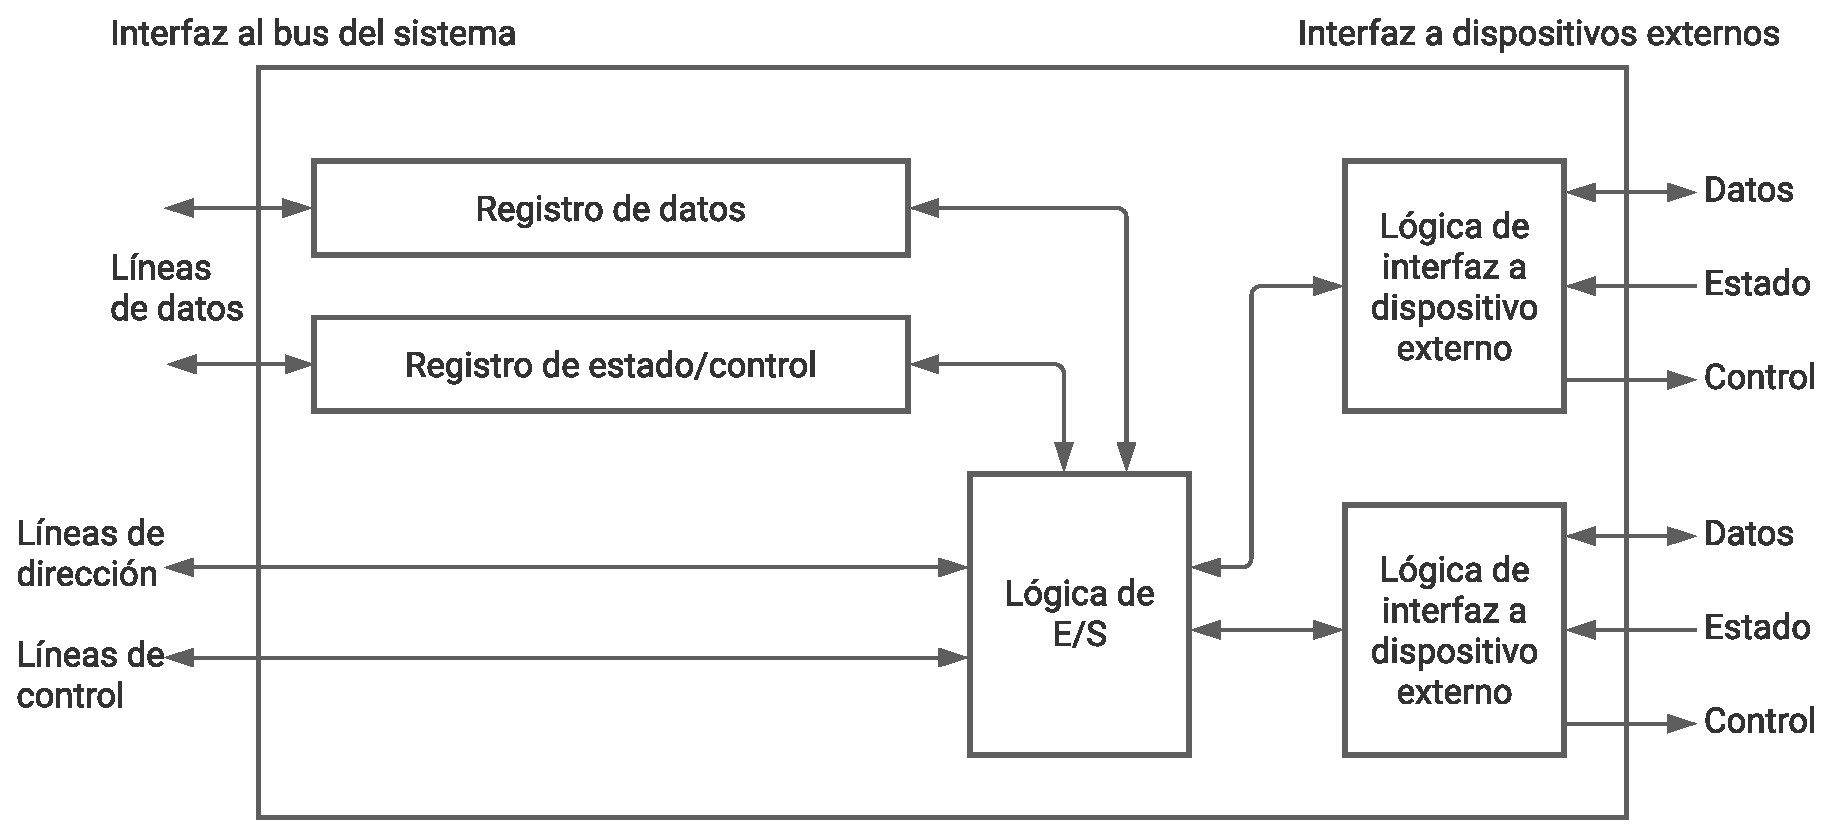
\includegraphics[width=0.6\textwidth]{Modulo-IO}
  \caption{Estructura de un módulo de E/S}\label{fig:Estructura-modulo-E/S}
\end{figure}

\subsection{Entrada y salida programada}

Los datos se intercambian entre el procesador y el módulo de E/S. El procesador ejecuta un programa que controla directamente la operación de E/S:\@
\begin{itemize}
  \item Comprobación del estado del dispositivo.
  \item Envío de una orden de lectura o escritura.
  \item Transferencia del dato.
\end{itemize}

El procesador espera que el módulo de E/S termine la operación.

Los detalles de la E/S programada se muestran en la Figura~\ref{fig:E/S-programada}:

\begin{itemize}
  \item La CPU solicita la operación de E/S.
  \item El módulo E/S realiza la operación.
  \item El módulo E/S activa los bits de estado del dispositivo direccionando y espera.
  \item La CPU comprueba periódicamente el estado de esos bits, hasta que detecta que la operación fue completada.
  \item En caso contrario la CPU espera y vuelve a comprobarlo más tarde.
\end{itemize}

\begin{figure}[h]
  \centering
  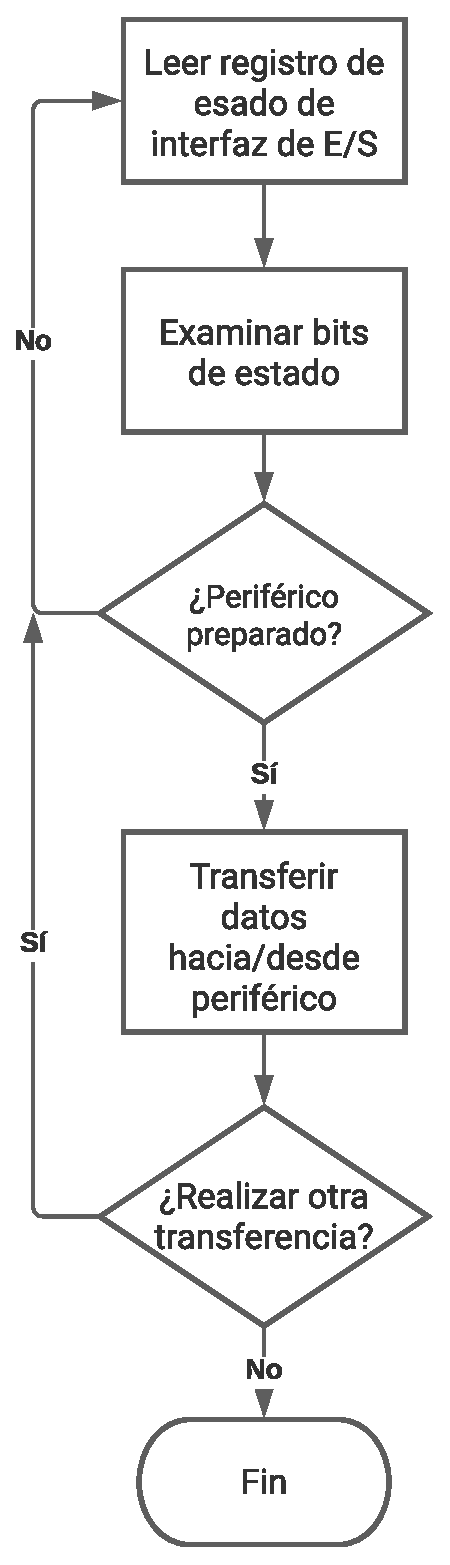
\includegraphics[height=0.38\textheight]{IO-programada}
  \caption{E/S programada}\label{fig:E/S-programada}
\end{figure}

\begin{subs}

  \subsubsection{Órdenes de E/S}
  Al ejecutar una instrucción relacionada con una E/S, el procesador proporciona una dirección, especificando el módulo de E/S particular y el dispositivo externo, y una orden de E/S. Hay cuatro tipos de órdenes de E/S que puede recibir un módulo de E/S cuando es direccionado porel procesador:

  \begin{itemize}
    \item \textbf{Control}: se utiliza para activar el periférico e indicarle qué hacer. Estas órdenes son específicas del tipo particular de periférico.
    \item \textbf{Test}: se utiliza para comprobar diversas condiciones de estado asociadas con el módulo de e/S y sus perífericos.
    \item \textbf{Lectura}: hace que el módulo de E/S capte un dato de un periférico y lo sitúe en un buffer interno. Después el procesador puede obterner el dato solicitando que el módulo de E/S lo ponga en el bus de datos.
    \item \textbf{Escritura}: hace que el módulo de E/S capte un dato del bus de datos y posteriormente lo transmita al periférico.
  \end{itemize}

\end{subs}

\subsection{Entrada y salida con interrupciones}

El problema con la E/S programada es que el procesador tiene que esperar un tiempo considerable a que el módulo de E/S en cuestión esté preparado para recibir o transmitir los datos.

En la E/S con interrupciones, el módulo de E/S interrumpirá al procesador para solicitar su servicio cuando esté preparado para intercambiar datos con él.


Desde el punto de vista del procesador, las acciones son las que siguen:

\begin{itemize}
  \item Envia una orden READ de lectura. El módulo E/S obtiene los datos del periférico mientras la CPU realiza otro trabajo.
  \item La CPU chequea si hay pedidos de interrupciones pendientes al final de cada ciclo de instrucción.
  \item La CPU detecta el pedido, guarda el contexto, interrumpe el proceso y realiza la gestión de la interrupción.
  \item La CPU solicita los datos. El módulo E/S transfiere los datos.
\end{itemize}

\begin{subs}
  \subsubsection{Cuestiones de diseño}

  En la implementación de las E/S mediante interrupciones aparecen dos cuestiones. Primero, cómo determina el procesador qué dispositivo ha provocado la interrupción. Y segundo, si se han producido varias interrupciones, como decide el procesador la que debe atender.

  Hay cuatro tipos de técnicas que se utilizan comunmente:

  \begin{itemize}
    \item \textbf{Múltiples línesas de interrupción}: consiste en proporcionar varias líneas de interrupción entre el procesador y los módulos de E/S. No resulta práctico dedicar más de unas pocas líneas del bus o terminales del procesador a ser líneas de interrupción.
    \item \textbf{Software poll}: cuando el procesador detecta una interrupción, se produce una bifurcación a una rutina de servicio de interrupción que se encarga de consultar cada módulo de E/S para determinar cuál ha provocado la interrupción. Este método es muy lento y no es muy eficiente.
    \item \textbf{Daisy chain}: es una alternativa a la técnica anterior. Todos los módulos de E/S comparten una línea común para solicitar interrupciones. La línea de reconocimiento de interrupción se conecta encadenando los módulos uno tras otro. Cuando el procesador recibe una interrupción, activa el reconocimiento de interrupción. Esta señal se propaga a trabés de la secuencia de módulos de E/S ahsta que se alcanza un módulo que solicitó la interrupción. El módulo respondera colocando un vector, en el bus, que lo identifica. La CPU emplea el vector como puntero para acceder a la rutina de servicio.
    \item \textbf{Arbitraje de bus}: un módulo de E/S debe en primer lugar disponer del control del bus antes de poder actibar la línea de petición de interrupción. Así, solo un módulo puede activar la línea en un mismo instante. Cuando el procesador detecta la interrupción, responde mediante la línea de reconocimiento de interrupción. Después, el módulo que solicitó la interrupción sitúa su vector en las línes de datos.
  \end{itemize}
\end{subs}

\subsection{Acceso directo a memoria}

El DMA requiere un módulo adicional en el bus del sistema. El módulo o controlador de DMA es capaz de imitar al procesador y de recibir el control del sistema cedido por el procesador. El módulo de DMA utiliza sólo cuando el procesador no lo necesita, o debe forzar al procesador a que suspenda temporalmente su funcionamiento. Esta última técnica es la más común y se denomina \textit{robo de cilo}.

Cuando el procesador desea leer o escribir un bloque de datos, envía una orden al módulo de DMA, incluyendo la siguiente información:

\begin{itemize}
  \item Si se solicita una lectura o una escritura, utilizando la línea de control de lectura o escritura el procesador y el módulo de DMA.\@
  \item La dirección del dispositivo de E/S en cuestión, indicada a través de las lías de datos.
  \item La posición inicial de memoria a partir de donde se lee o se escribe indicada a través de las lineas de datos y almacenada por el módulo de DMA en su registro de direcciones.
  \item El número de palabras a leer o escribir, también indicando a través de las líneas de datos y alamacenado en el registro de cuenta de datos.
\end{itemize}

El procesador delega la operación de E/S al módulo de DMA, que se encargará de ella. El módulo de DMA transfiere el bloque completo de datos, directamente desde o hacia la memoria, sin que tenga que pasar a través del procesador. Una vez que la transferencia termina, el módulo de DMA envía una señal de interrupción al procesador.

Para una transferencia de E/S de varias palabras, el DMA es mucho más eficiente que la E/S mediante interrupciones o la E/S programada.

Aunque la transferencia por DMA puede ser más eficientes, puede haber ciertos problemas. Se puede degradar el rendimiento de la CPU si el DMA hace uso intensivo del bus.

El problema se reduce con el uso de memoria cache. La mayor parte del tiempo, la CPU lee instrucciones de la cache por lo que no necesita usar el bus de memoria. El DMA puede aprovechar estos intervalos en los que la CPU está leyendo instrucciones de la cache para realizar las transferencias.

En caso de computadores sin cache, el procesador no utiliza el bus en todas las fases de la ejecución de una instrucción. El DMA puede aprovechar las fases de ejecución de una instrucción en las que la CPU no utiliza el bus para realizar sus transferencias.

Si el DMA sólo toma el control del bus durante los intervalos de tiempo en los que la CPU no hace uso del mismo el rendimiento del sistema no sufrirá degradación alguna

Si pueden distinguir dos tipos de transferencias:

\begin{itemize}
  \item Por ráfagas
  \item Por robo de ciclo
\end{itemize}

\begin{subs}
  \subsubsection{DMA modo ráfaga}

  Cuando la CPU concede el bus, el DMA no lo libera hasta haber finalizado la transferencia de todo el bloque de datos completo. La ventaja que tiene es que la transferencia se realiza de forma rápida. Pero la desventa es que durante el tiempo que dura la transferencia la CPU no puede utilizar el bus con memoria, lo que puede degradar el rendimiento del sistema.

  \subsubsection{DMA modo robo de ciclo}

  Cuando la CPU concede el bus al DMA, se realiza la transferencia de una única palabra y después el DMA libera el bus. El DMA solicita el control del bus tantas veces como sea necesario hasta finalizar la transferencia del bloque completo.

  La ventaja que tiene es que no se degrada el rendimiento del sistema. Aunque por contraparte, la transferencia tarda más tiempo en llevarse a cabo.

  Para la CPU no es considerado una interrupción, por lo que no es necesario guardar el contexto. Si bien el trabajo de la CPU es lento, no será tanto como si ella realizara la transferencia. Por lo tanto, para transferencia de E/S de múltiples palabras, es la técnica más eficiente.

\end{subs}

\subsection{Canales de E/S}

A medida que los computadores han evolucionado, la complejidad y sosfiticación de sus componentes se ha incrementado. En ningún lugar se hace más evidente que en el funcionamiento de las E/S. Sus etapas pueden resumirse como:

\begin{enumerate}
  \item La CPU controla directamente los periféricos.
  \item Se agrega un módulo de E/S o controlador.
  \item Idem 2, más llamado de interrupción.
  \item El módulo de E/S provee el acceso directo a memoria(DMA).
  \item El módulo de E/S tiene su propio procesador con su pequeño conjunto de instruccioens.
  \item El módulo además tiene su memoria local, (se convierte en una computadora en sí mismo).
\end{enumerate}




\appendix

\section{Pilas}\label{ap:pilas}

Una \textbf{pila} es un conjunto ordenado de elementos, en el que solo uno de ellos es accesible en un instante dado. El punto de acceso se denomina \textit{cabecera} de la pila. El número de elementos en la pila, se denomina \textit{longitud}. Es una estructura de tipo \textit{LIFO} (Last In First Out), es decir, el último elemento en entrar es el primero en salir.

\begin{figure}[h]
  \centering
  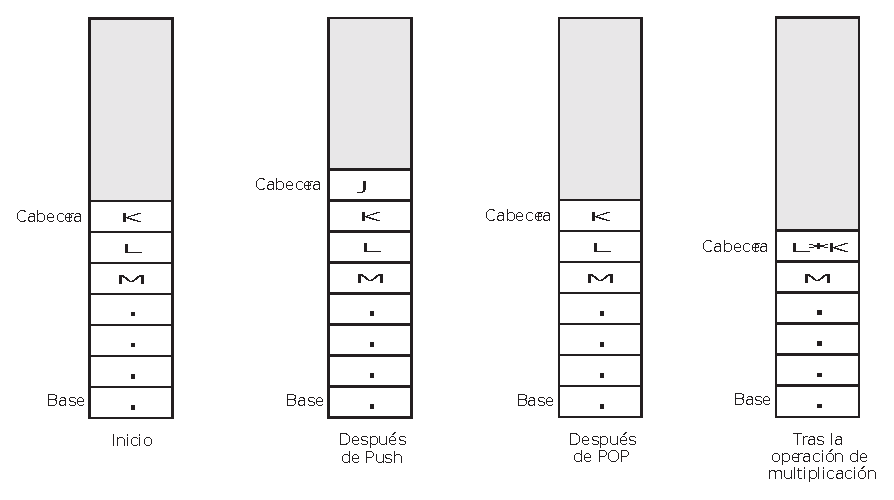
\includegraphics[width=0.8\textwidth]{Pila}
  \caption{Pila}
\end{figure}

La pila es una estructura útil como parte de la implementación del procesador. Por ejemplo, en el procesamiento de llamadas a subrutinas, la pila se utiliza para almacenar la dirección de retorno de la subrutina.

La implementación de una pila requiere que exista un cierto conjunto de posiciones utilizadas para almacenar los elementos de la pila.En memoria principal se reserva un bloque de posiciones contiguas para la pila.
Para un funcionamiento correcto se necesitan tres direcciones, normalmente memorizadas en registros del procesador:

\begin{itemize}
  \item \textbf{Stack pointer (SP)}: contiene la dirección del tope o cabecera de pila.
  \item \textbf{Stack base (SB)}: contiene la dirección de la base de la pila.
  \item \textbf{Stack limit (SL)}: contiene la dirección de la ultima posición reservada de la pila.
\end{itemize}
\section{Interfaces de espacio}

Hay 2 métodos para hacer la interfaz del espacio de E/S:\@

\subsection*{E/S aislado}

Esta técnica es utilizada por sistemas basados en procesadores Intel. En este tipo de interfaz, las posiciones de E/S se encuentran separadas de la memoria principal, en un espacio distinto de direcciones. Las direcciones de E/S llamadas puertos, están separadas de la memoria.

La principal ventaja de esta técnica es que todo el espacio de memoria se encuentra ocupado por la misma. La desventaja es que para transferir datos entre el $\mu p$ y E/S se tienen que usar instrucciones especiales como IN y OUT.\@

Cuando la UC decodifica OUT ó IN, activa las líneas del bus de control iow=input/output write ó ior=input/output read.

Cuando la UC decodifica MOV, activa las líneas del bus de control mwr=memory write ó mrd=memory read.

\subsection*{E/S mapeada en memoria}

En esta técnica, las direcciones de E/S están mapeadas en las direcciones de memoria, por lo que las direcciones de E/S pertenecen al espacio de memoria. La principal ventaja es que se puede usar todo el conjunto de instrucciones del procesador, porque todas las posiciones son tomadas como direcciones. La desventaja es que el espacio de memoria se ve reducido por la presencia de las direcciones de E/S.
\section{PIO}

Son 2 puertos paralelos de 8 bits: A y B. Se puede programar con bits por separados como entrada ó salida. Posee 4 registros internos de 8 bits cada un: 2 de datos, PA y PB;\@ 2 de control, CA y CB.\@ 

Un bit en 0 en el registro CA selecciona como salida a la línea correspondiente de PA.\@ Un bit en 1 en el registro CA selecciona como entrada a la línea correspondiente de PA.\@ Los bits en CB controlan de la misma manera al registro PB.\@

\end{document}
